\documentclass[a4paper, 12pt]{report}

%%%%%%%%%%%%
% Packages %
%%%%%%%%%%%%

\usepackage[english]{babel}
\usepackage[noheader]{packages/sleek}
\usepackage{packages/sleek-title}
\usepackage{packages/sleek-theorems}
\usepackage{packages/sleek-listings}

% Per figure nel testo
\usepackage{wrapfig}

% Per aggiungere ``Page 1 of 100''
\usepackage{lastpage}

%\cfoot{\thepage\ of \label{LastPage}}
\cfoot{Page \thepage \hspace{1pt} of \pageref{LastPage}}

%%%%%%%%%%%%%%
% Title-page %
%%%%%%%%%%%%%%

\logo{./resources/img/logo.png}
\institute{Ca' Foscari University}
\faculty{Faculty of Computer Science}
%\department{Department of Anything but Psychology}
\title{Cryptography}
\subtitle{Afternotes}
\author{\textit{Author}\\Francesco \textsc{Vivian}}
%\supervisor{Linus \textsc{Torvalds}}
%\context{Well, I was bored...}
\date{A.Y. 2020-2021}

%%%%%%%%%%%%%%%%
% Bibliography %
%%%%%%%%%%%%%%%%

\addbibresource{./resources/bib/references.bib}

%%%%%%%%%%
% Others %
%%%%%%%%%%

\lstdefinestyle{latex}{
    language=TeX,
    style=default,
    %%%%%
    commentstyle=\ForestGreen,
    keywordstyle=\TrueBlue,
    stringstyle=\VeronicaPurple,
    emphstyle=\TrueBlue,
    %%%%%
    emph={LaTeX, usepackage, textit, textbf, textsc}
}

\FrameTBStyle{latex}

\def\tbs{\textbackslash}

%%%%%%%%%%%%
% Document %
%%%%%%%%%%%%

\newtheorem{definition}{\textbf{Definition}}
\newtheorem{property}{\textbf{Property}}
\newtheorem{example}{\textbf{Example}}

\begin{document}
    \maketitle
    %\romantableofcontents
\chapter*{Lecture 1}
\begin{definition}
	Security: it generically refers to the possibility of "protecting" information, which is either stored in a computer system or transmitted on a network.
\end{definition}
Whatever will be shown works in both situations.\\
To decide whether a computer system is "secure", you must first decide what secure means to you, then identify the threats you care about. Some threats are: cyberterrorism, denial of service, modified databases, virus, identity theft, stolen customer data, equipment theft, espionage.

\vspace{5mm}
There are different aspects to protect through security properties:
\begin{property}
	Authenticity: an entity should be correctly identified.
\end{property}
\begin{example}
	Some examples of authenticity:
	\begin{itemize}
		\item login process for authenticating a user (User Identification)
		\item a digital signature allows for authenticating the entity originating a message (Message Authentication)
	\end{itemize}
\end{example}
\vspace{5mm}
\begin{property}
	Confidentiality (secrecy): information should only be accessed (read) by authorized entities.
	\begin{itemize}
		\item Confidential information is not disclosed to unauthorized individuals (Data confidentiality)
		\item Individuals control what information related to them may be collected and stored and by whom that information may be disclosed (Privacy)
	\end{itemize}
\end{property}
\begin{example}
	Some examples of confidentiality:
	\begin{itemize}
		\item the person that accesses a database should be authorized to access the data
		\item personal privacy, my private data should be protected while browsing the web
	\end{itemize}
\end{example}
The "access control" for confidentiality:
\begin{itemize}
	\item use the "need to know" basis for data access. How do we know who needs what data? (Approach: access control specifies who can access what). How do we know a user is the person she claims to be? We need her identity and we need to verify this identity (Approach: identification and authentication).
	\item Analogously, the "need to access/use" is the basis for access to physical assets (access to a computer room, use of a desktop)
\end{itemize}
Confidentiality is difficult to ensure and easy to assess in terms of success: it is binary in nature (Yes/No).
\vspace{5mm}
\begin{property}
	Integrity: information should only be modified by authorized entities.
	\begin{itemize}
		\item information and programs are changed only in a specified and authorized manner (Data integrity)
		\item a system performs its intended function, free from unauthorized manipulation (System integrity)
	\end{itemize}
\end{property}
\begin{example}
	We should not alter bank accounts and IoT device firmware.
\end{example}
If we don't have integrity, we also don't have confidentiality (with integrity I want only authorized users to be able to modify information, with confidentiality I want only authorized users to be able to see information, modifying includes seeing).
Integrity is more difficult to to measure than confidentiality, it is non binary (it has degrees of integrity) and it is content-dependent (it means different things in different context)
\begin{example}
	A quotation from a politician, we can preserve the quotation (data integrity) but mis-attribute (origin integrity), like \textit{Y said that} instead of \textit{X said that}. 
\end{example}
\vspace{5mm}
\begin{property}
	Availability: information should be available/usable fastly by authorized users.
\end{property}
\begin{example}
	It is important to guarantee reliability and safety. Apart from attacks, availability might be loss in case of faults (we need to use fault-tolerant techniques). We need availability in case of a remote surgery for example (good QoS).
\end{example}
We can say that an asset (a resource) is available if:
\begin{itemize}
	\item it provides a timely request response
	\item it provides fair allocation of resources (no starvation)
	\item it is fault tolerant (no total breakdown)
	\item it is easy to use in the intended way
	\item it provides controlled concurrency (concurrency control, deadlock control, ..)
\end{itemize}
\vspace{5mm}
\begin{property}
	Non-repudiation: an entity should not be able to deny an event. 
\end{property}
\begin{example}
	Having sent/received a message. This property is crucial for e-commerce, where "contracts" should not be denied by parties.
\end{example}
\vspace{5mm}
Other properties that are not addressed in detail are: fairness of contract signing, privacy, anonimity and unlinkability, accountability, ..
\subsubsection{Typical attacks}
We will now see some typical attacks. We assume that information is flowing from a source to a destination (e.g.: reading data is a flow from the data container to a user, writing is a flow from a user to the file system).\\

\begin{wrapfigure}[9]{l}{0.4\textwidth}
	%\centering
	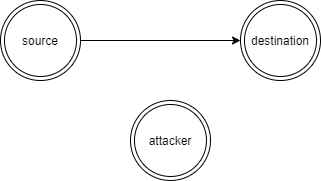
\includegraphics[width=0.37\textwidth]{images/attacks1.png}
	\caption{Expected information flow}
	\label{fig:attacks1}
\end{wrapfigure}
Malicious users might try to subvert the properties previously mentioned in many different ways. We will now give a general classification depending on how an attacker might interfere on the expected flow of information (Figure \ref{fig:attacks1}).

\begin{wrapfigure}[5]{r}{0.4\textwidth}
	%\centering
	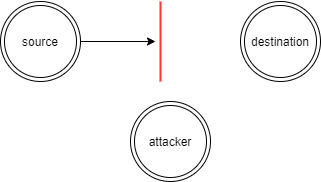
\includegraphics[width=0.37\textwidth]{images/attacks2.png}
	\caption{The attacker interrupts the flow of information}
	\label{fig:attacks2}
\end{wrapfigure}

\begin{definition}
	Interruption: the attacker stops the flow of information (Figure \ref{fig:attacks2}). The attacker interrupts a service, it breaks system integrity and availability.
\end{definition}

\vspace{5mm}
Some examples of interruption:
\begin{example}
	\leavevmode
	%Some examples of interruption:
	\begin{itemize}
		\item the destruction of a part of the hardware
		\item canceling of programs or data files
		\item the destruction of a network link
		\item a denial of service (DoS) that makes the system/network unusable 
	\end{itemize}
\end{example}

\begin{wrapfigure}[6]{l}{0.4\textwidth}
	%\centering
	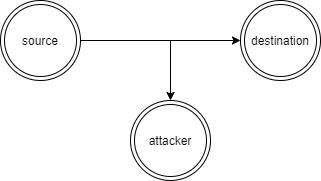
\includegraphics[width=0.37\textwidth]{images/attacks3.png}
	\caption{The attacker intercepts information}
	\label{fig:attacks3}
\end{wrapfigure}

\begin{definition}
	Eavesdropping (interception): the attacker gets unauthorized access to the information (depicted as an additional flow towards the attacker).
\end{definition}

\vspace{5mm}
Interception is an attack to confidentiality, these attacks are hard to detect.
\begin{example}
	\leavevmode
	\begin{itemize}
		\item unauthorized copies of files or programs;
		\item interception of data flowing in the network (a credit card number).
	\end{itemize}
\end{example}
\vspace{15mm}
Interception attacks are hard to detect because source and destination don't notice any change (differently from interruption, where destination don't receive the flow).


\begin{wrapfigure}[6]{l}{0.4\textwidth}
	%\centering
	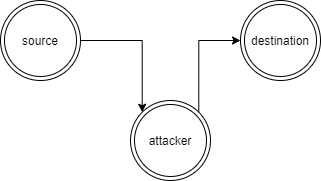
\includegraphics[width=0.37\textwidth]{images/attacks4.png}
	\caption{The attacker modifies information}
	\label{fig:attacks4}
\end{wrapfigure}

\begin{definition}
	Modification: the attacker intercepts the information and make unauthorized modification.
\end{definition}

In this case destination might notice that something is wrong.
\begin{example}
	\leavevmode
	\begin{itemize}
		\item unauthorized change of values (e.g.: of a database);
		\item unauthorized change of a program;
		\item unauthorized change of data flowing in a network;
		\item \texttt{A} redirects \texttt{S}'s bank transfer to herself (either in the browser or in the network, man in the middle).
	\end{itemize}
\end{example}

\begin{wrapfigure}[5]{r}{0.4\textwidth}
	%\centering
	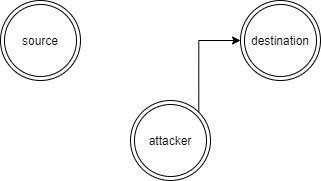
\includegraphics[width=0.37\textwidth]{images/attacks5.png}
	\caption{The attacker forges new information}
	\label{fig:attacks5}
\end{wrapfigure}

\begin{definition}
	Forging (falsification): the attacker inserts new information in the system (usually related to impersonation since the attacker lets the destination believe the information is coming from the honest source). 
\end{definition}

Forging is an attack to \textit{authenticity, accountability} and \textit{integrity}.

\begin{example}
	\leavevmode
	\begin{itemize}
		\item addition of messages in the network;
		\item addition of a record in the database.
	\end{itemize}
\end{example}

\vspace{35mm}

\begin{figure}[H]
	\centering
	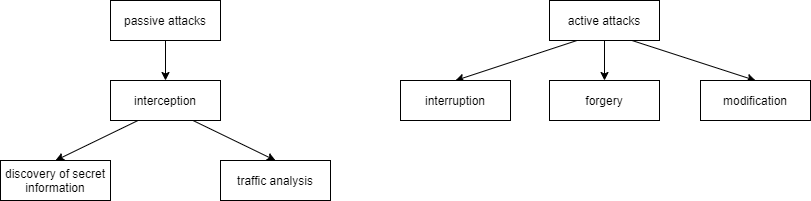
\includegraphics[scale=0.55]{images/typeofattacks.png}
	\caption{Classification of different types of attacks}
	\label{fig:typeofattacks}
\end{figure}
\newpage
\begin{example}
	Suppose a bank B is using the following simple protocol to allow a bank transfer from user Alice (A):\\
	\begin{center}
	\texttt{A $\rightarrow$ B: sign\_A("}please pay Bob 1000€\texttt{")}
	\end{center}
	\texttt{sign\_A} is some "signature" mechanism to ensure that the message really comes from Alice (thus the attacker cannot generate valid signed messages from Alice).
	
	Let's suppose Bob is the attacker, he intercepts the whole message and repeats it as many times as he want, without modifying it. This attack (called replay) consists of an interception plus forging (in this case the message is just re-sent as it is). Bob obtains many bank transfers by just re-sending message M.
\end{example}

\begin{example}
	Program modification: It is an attack to confidentiality, Bob modifies a program that is used by Alice, such a program apparently works normally, however it changes (e.g. the access rules of the users that are executing it, in this case it is called \textit{Trojan horse}). Bob waits that Alice uses the program and copies all the files of Alice in his home directory.
\end{example}

\subsubsection{Cryptography}
The term \textit{cryptography} comes from the greek and means "hidden writing". It is a way to protect the information when the environment is insecure.
For example it is used when the information is sent on a network such as internet or when the system does not support sufficient protection mechanisms.

\begin{definition}
	Encryption: a \textit{plaintext} (message) is transformed using some rules (encryption algorithm) in a ciphertext.
\end{definition}

\begin{definition}
	Decryption: the plaintext is reconstructed starting from a ciphertext.
\end{definition}

The decryption has to be simple for the receiver and unfeasible for an attacker.
The information is encrypted in the source and travels to the destination where it will be decrypted.
In order to do this there are two possible solutions:
\begin{enumerate}
	\item only the sender (Alice) and the receiver (Bob) know the encryption algorithm. If the attacker, by looking at the flow of information, is able to guess which algorithm is used, then he will be able to decrypt all the messages sent;
	\item the encryption algorithm is public and Alice and Bob share some information (the encryption key) non accessible by the attacker. If the attacker doesn't have the encryption key, it is unfeasible to decrypt the messages.
\end{enumerate}

The second solution is better because it is simpler to distribute only one key and if there is an attack it is easier to change key instead of a whole algorithm.

\begin{figure}[H]
	\centering
	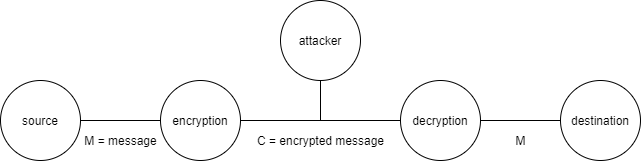
\includegraphics[scale=0.6]{images/enc1.png}
	\caption{Encryption with a shared key}
	\label{fig:enc1}
\end{figure}

We want to build a secure channel to be able to exchange the encryption key.

\begin{figure}[H]
	\centering
	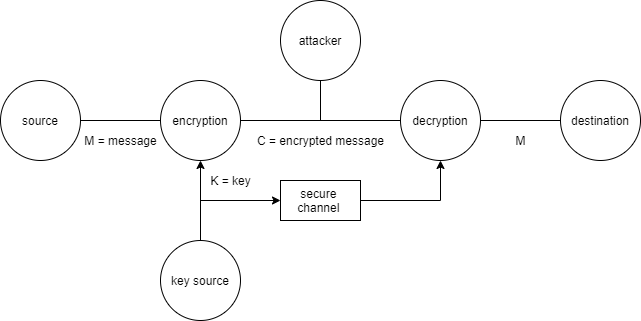
\includegraphics[scale=0.6]{images/enc2.png}
	\caption{Encryption with a shared key and the secure channel}
	\label{fig:enc2}
\end{figure}

This is called \textit{symmetric key cipher} (symmetric because source and destination use the same key).

One of the first encryption algorithms was used by Julius Caesar. In the Caesar Cipher all the letters are permuted using a certain rule (each letter is substituted by the one 3 positions ahead in the alphabet)

\begin{center}
	\texttt{A $\rightarrow$ D\\
	B $\rightarrow$ E\\
	C $\rightarrow$ F\\
	...\\
	Z $\rightarrow$ C}
\end{center}

In this case the algorithm is the Caesar Cipher and the key is 3.
\end{document}
